\documentclass[../../report.tex]{subfiles}
\begin{document}
\section{Musicality}

The previous sections evaluated the model's performance in terms of objective
but crude statistical metrics. For a generative model, good accuracy values are
not necessarily an indicator of perceptually satisfying results, so it is a good
idea to perform a manual reality check.

Objective evaluation of a work of music is arguably impossible. Its individual
qualities can be described, but it is up to the listener to decide whether those
qualities are pleasant or bothersome. That being said, there are a few very
general features of music that are thought to be universal, such as tonality,
theming, and a tendency towards smaller melodic intervals \cite{Mehr2019}.

\subsection{The bad}

The glaring issue with the model is its inability to stick to a consistent theme
throughout a melody. This is a known problem that is inherent in the simplistic
architecture of the Basic RNN model \cite{Abolafia2016}.

\begin{figure}[h]
  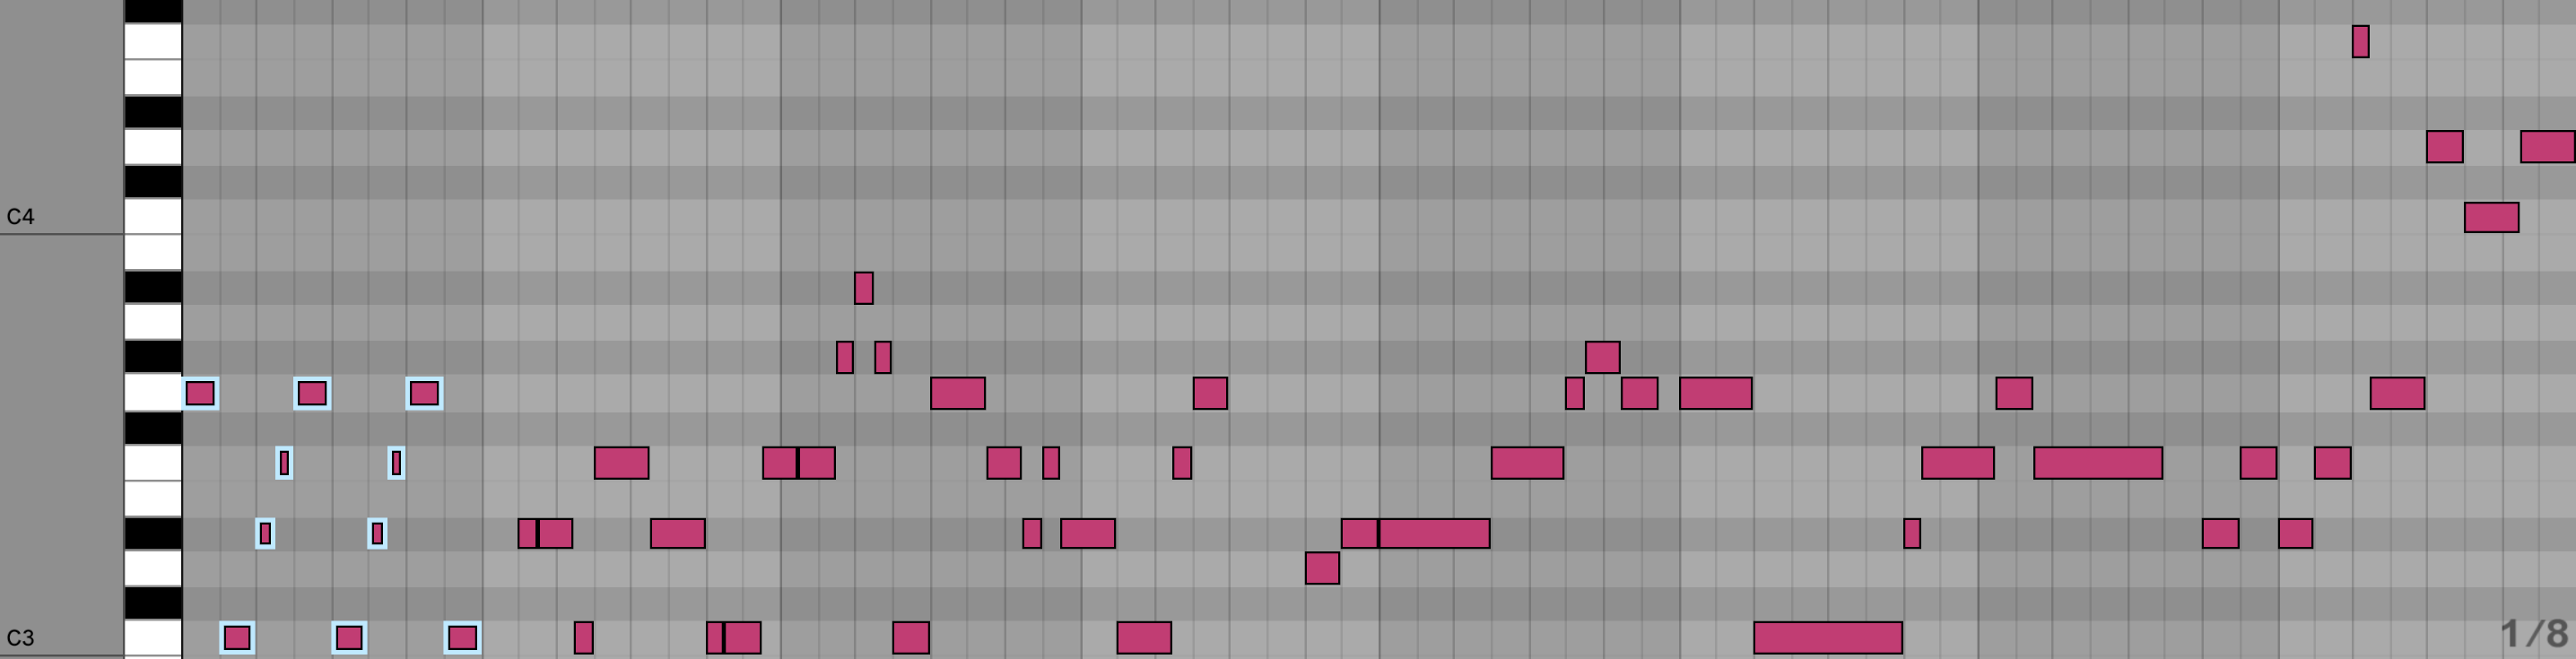
\includegraphics[width=\textwidth]{gen-got}
  \caption{When given one bar of the \emph{Game of Thrones} theme, the model
  seems to forget the pattern immediately.}
\end{figure}

\subsection{The good}

If we allow ourselves to ignore the lack of long-term structure and instead
focus on simpler features, we find that the model has actually learned a thing
or two.

\subsubsection{Tonality}
The model seems to have understood the concept of tonality. Most of the time, it
is able to stay in key.

\begin{figure}[h]
  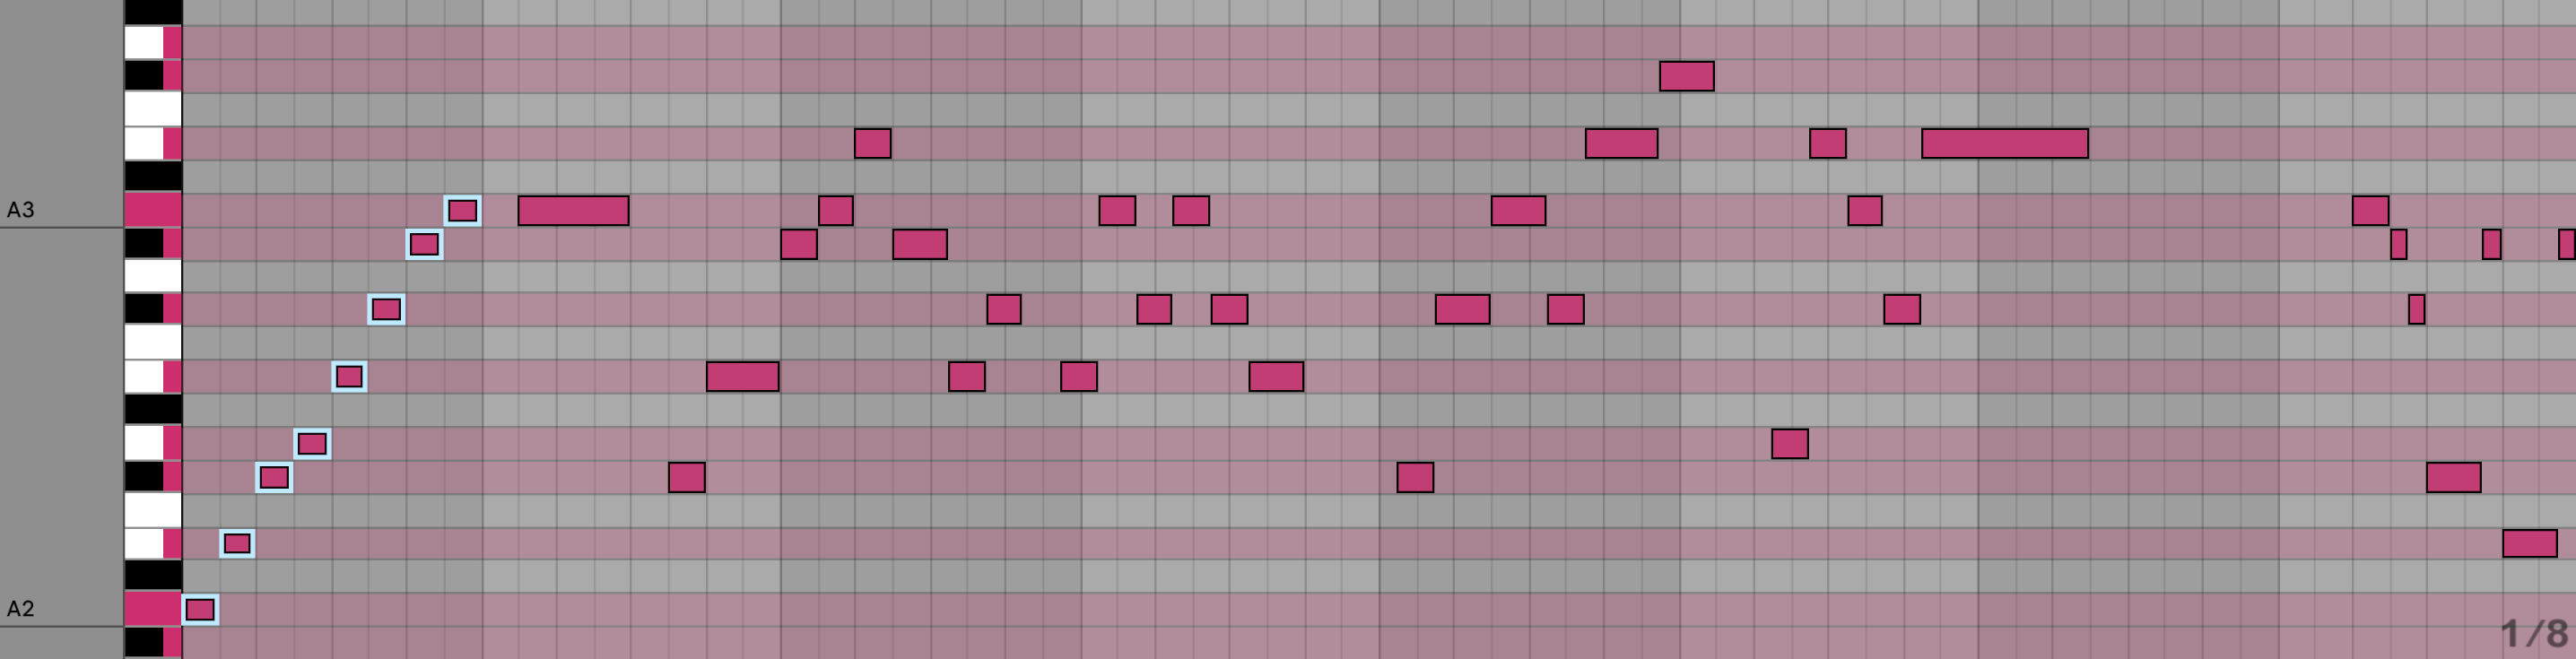
\includegraphics[width=\textwidth]{gen-amaj}
  \caption{When primed with an ascending A major scale, the model manages to
  continue playing in key throughout the whole sequence.}
\end{figure}

\subsubsection{Register consistency}
If the primer melody consists of notes purely in the upper or lower register,
the generated melody will tend to stay in the same register.

\begin{figure}[h]
  \begin{subfigure}[b]{\textwidth}
    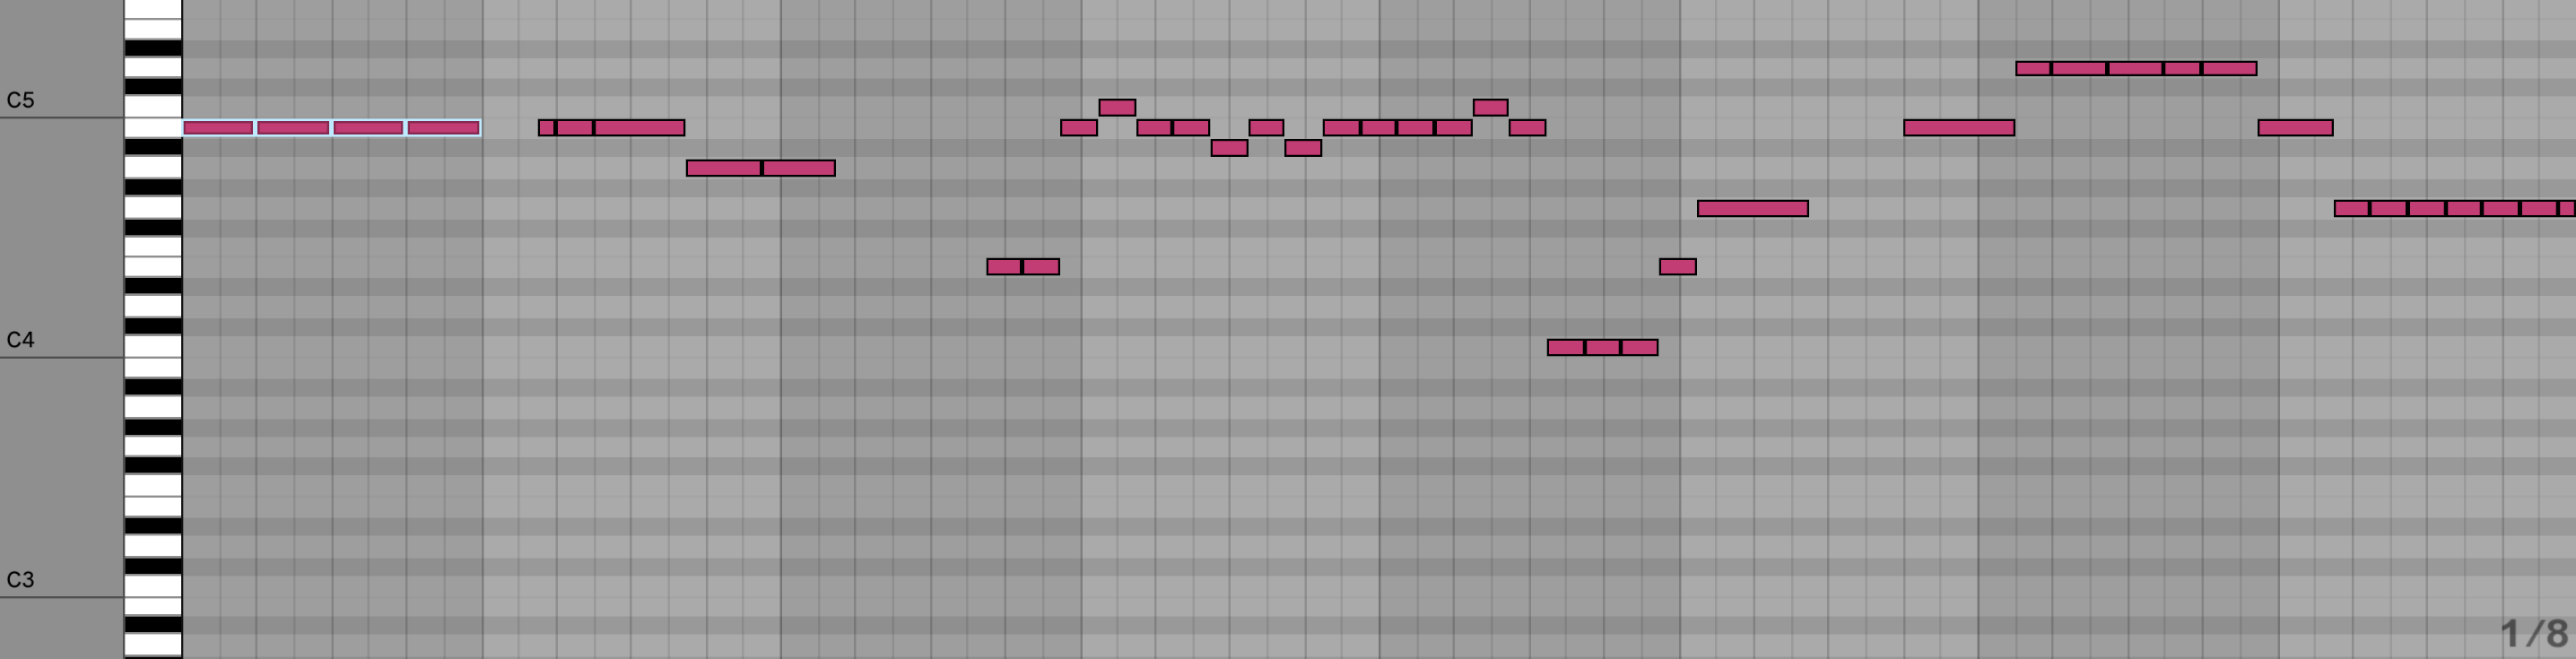
\includegraphics[width=\textwidth]{gen-high}
    \caption{Upper}
    \vspace{1mm}
  \end{subfigure}
  \begin{subfigure}[b]{\textwidth}
    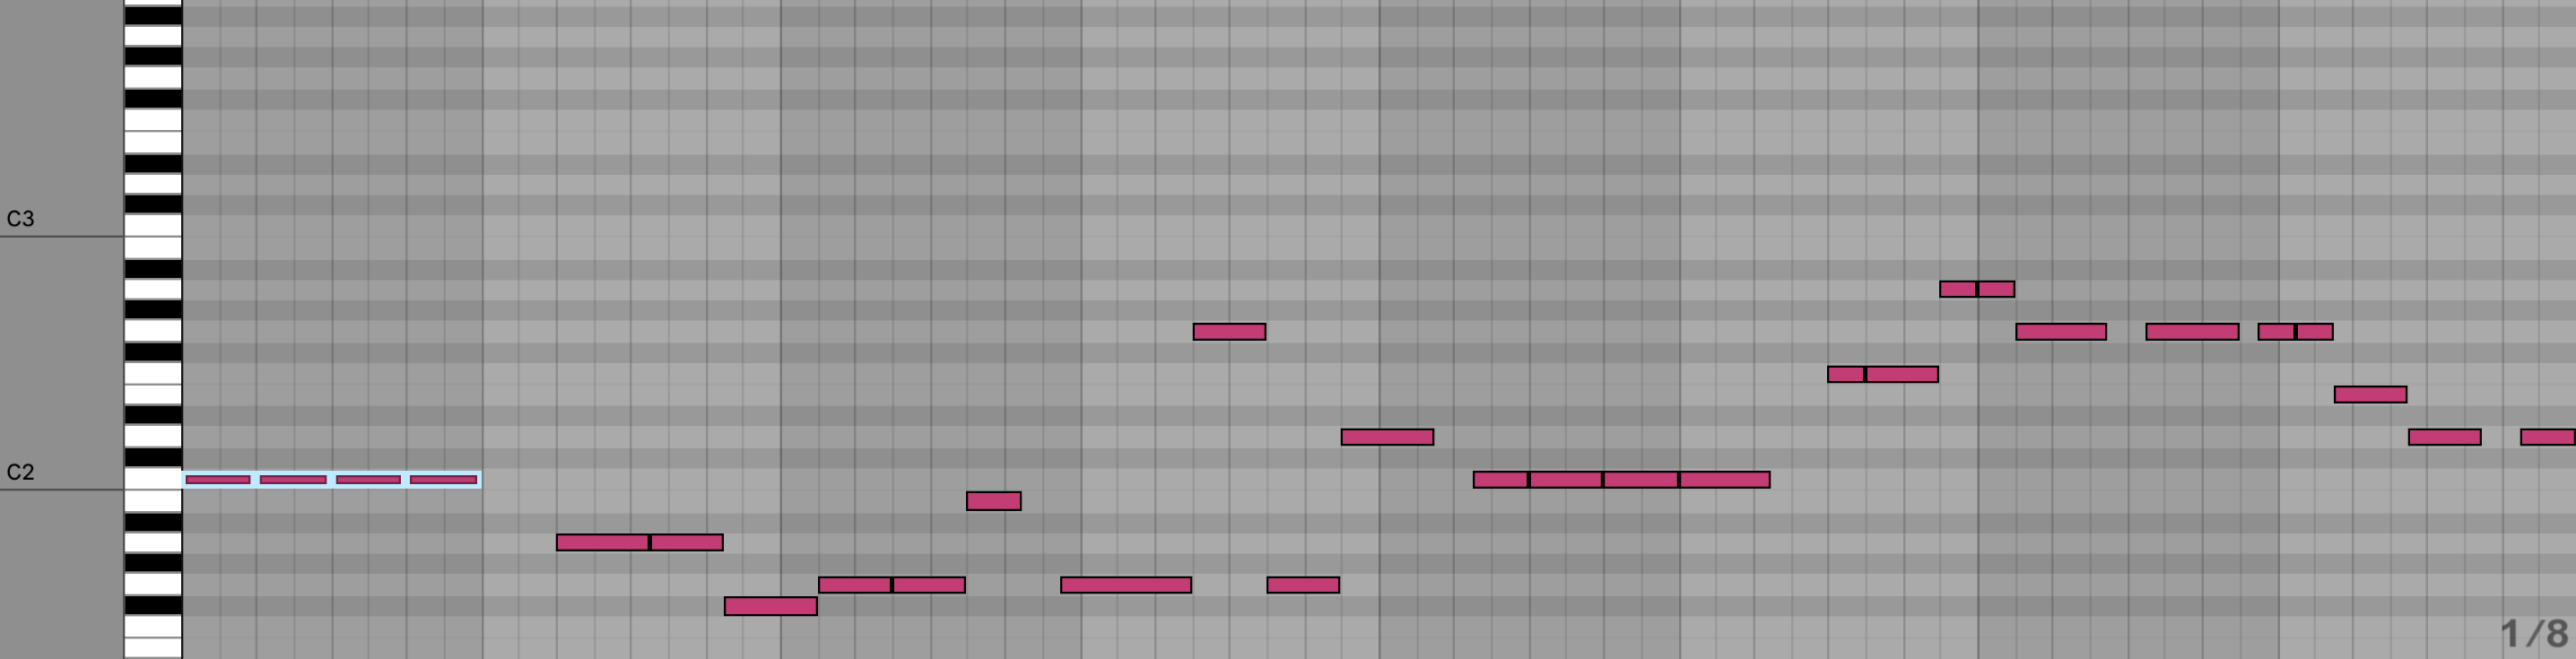
\includegraphics[width=\textwidth]{gen-low}
    \caption{Lower}
  \end{subfigure}
  \caption{Priming with sequences in different registers.}
\end{figure}

\subsubsection{Note density}
The model seems to pay attention to note duration in the primer melody. When
primed with many short notes, the generated melody is more energetic, while
priming with long notes results in a calmer melody.

\begin{figure}[h]
  \begin{subfigure}[b]{\textwidth}
    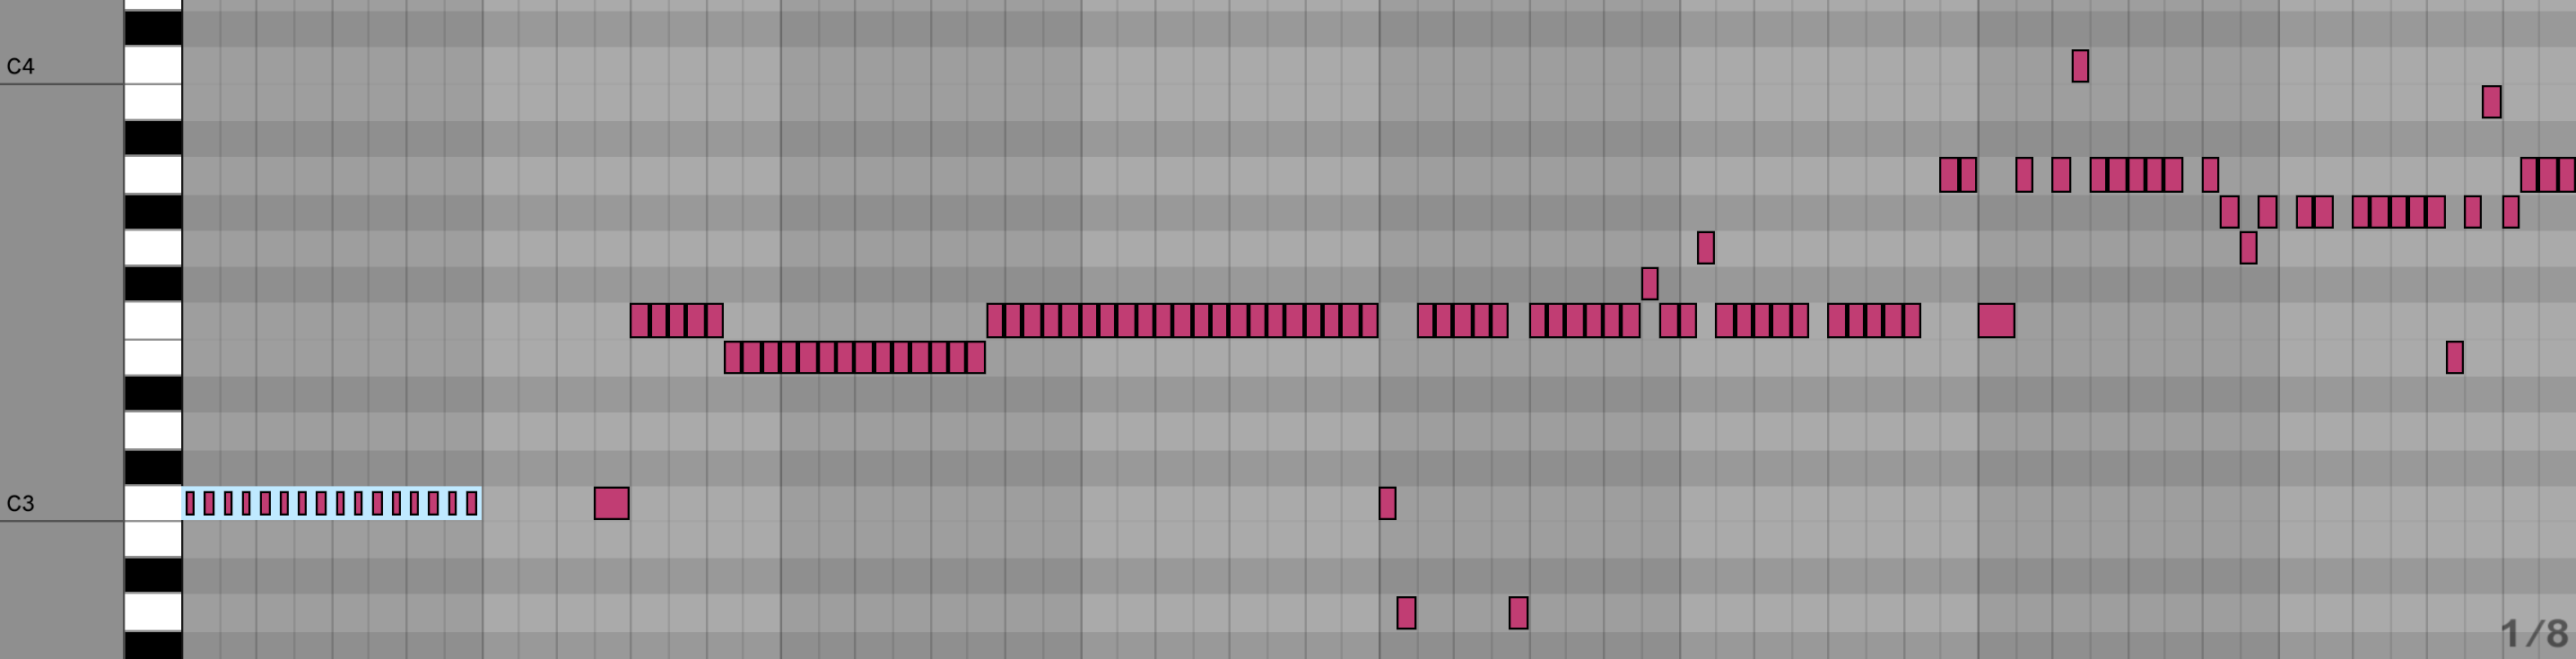
\includegraphics[width=\textwidth]{gen-fast}
    \caption{Sixteenth notes}
    \vspace{1mm}
  \end{subfigure}
  \begin{subfigure}[b]{\textwidth}
    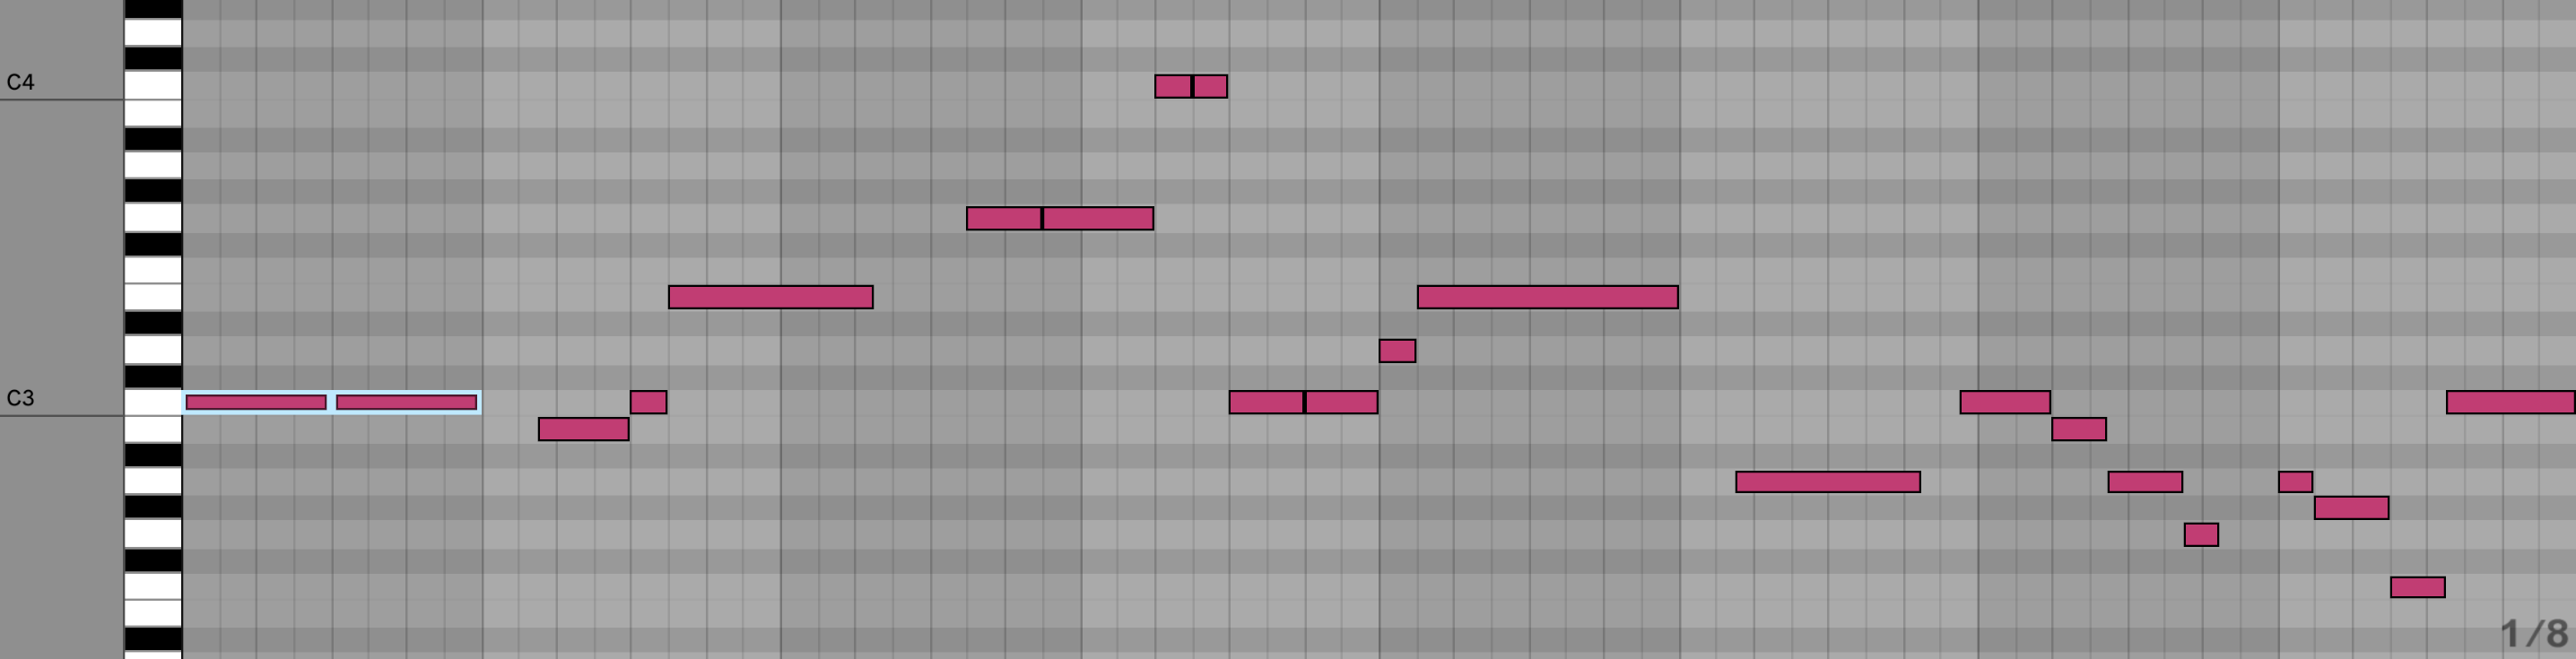
\includegraphics[width=\textwidth]{gen-slow}
    \caption{Half notes}
  \end{subfigure}
  \caption{Priming with sequences of different note duration.}
\end{figure}

\end{document}
